\documentclass[a4paper,12pt]{article}

% Packages
\usepackage{graphicx}
\usepackage{amsmath}
\usepackage{geometry}
\usepackage{fancyhdr}
\usepackage{setspace}
\usepackage{subcaption}
\usepackage{titlesec}  % For title formatting
\geometry{margin=1in}
\usepackage[utf8]{inputenc}
\usepackage{polski}
\usepackage{hyperref}
\usepackage{algpseudocode}
\usepackage{float}
\usepackage{dsfont}
\setstretch{1.2}

\DeclareMathOperator*{\argmin}{arg\,min}

% Header and Footer
\pagestyle{fancy}
\fancyhf{}
\fancyhead[L]{Klasyfikacja binarna}
\fancyhead[R]{\thepage}

% Title Formatting
\titleformat{\section}{\normalfont\Large\bfseries}{\thesection}{1em}{}

% Cover Page
\title{
    \vspace{2cm} % Adjust vertical space
    \begin{figure}[h!]
        \centering
        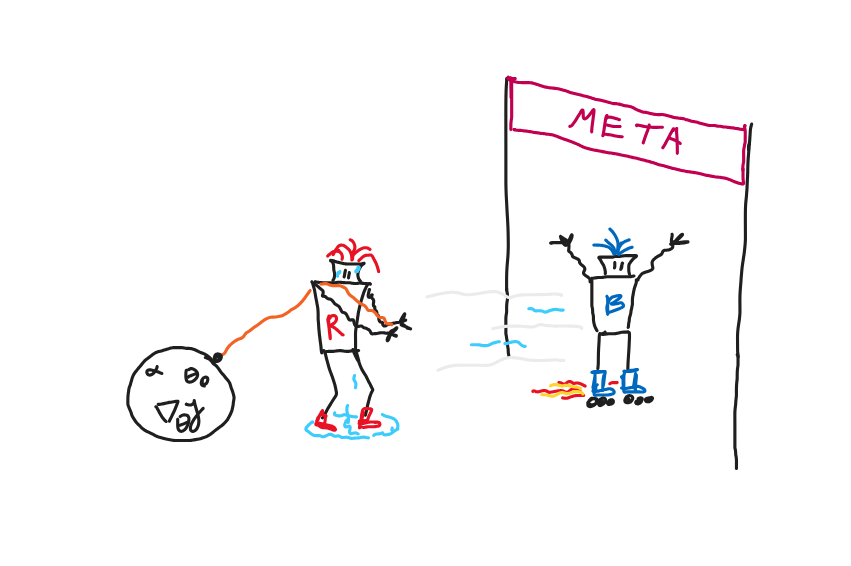
\includegraphics[width=0.8\textwidth]{title-drawing.png} 
        \caption{Tym razem to mój szkic}
    \end{figure}
    \vspace{1cm} % Adjust vertical space after the logo
    \textbf{\Huge Miniprojekt 2: Klasyfikacja binarna} \\
    \vspace{1cm} % Adjust vertical space
    \large Metody Probabilistyczne w Uczeniu Maszynowym \\
    \vspace{0.5cm} % Adjust vertical space
    \large \date{\today}
}
\author{Szymon Szulc}


\begin{document}

% Title Page
\maketitle
\thispagestyle{empty}
\newpage

% Table of Contents
% Start page numbering from the Table of Contents
\setcounter{page}{1}  % Start counting from 1
\tableofcontents
\newpage

\section{Wstęp}
Niniejszy raport oparty jest na notatniku \texttt{main.ipynb}. Raport ma stanowić zwięzłe i czytelne podsumowanie mojej pracy nad problemem klasyfikacji binarnej korzystając z naiwnego klasyfikatora bayesowskiego oraz regresji logistycznej.

\section{Badany problem}
\subsection{Definicja}
Dane to wyniki badań diagnostycznych pozwalających stwierdzać, czy wykryty rak piersi jest łagodny czy złośliwy. 
\subsection{Założenia}
Formalnie:
\begin{align*}
    &y \in \{2, 4\}, \hspace{22pt} \text{gdzie } y = 4 \text{ to rak złośliwy} \\
    &\forall j \in \{1,\dots,9\} \hspace{7pt} x_j \in \{1,\dots,10\}, \hspace{22pt} \text{mamy do czynienia z cechami dyskretnymi} \\
    &p(x_j = d | y = c) = \phi_{c,d}^j, \hspace{22pt} \text{gdzie } \sum_{d=1}^{10}{\phi_{c,d}^j} = 1 \\
    &\text{czyli zmienne } x_j|y=c \text{ mają rozkład wielomianowy}.
\end{align*}

\section{Pierwszy kontakt z danymi}
Mamy 9 cech -- $x_1,\dots, x_9$ i zmienną binarną $y$. Pierwsze co zrobiłem to \hyperref[fig:corr]{macierz korelacji}, którą znamy już z poprzedniego miniprojektu.

\begin{figure}[H]
    \centering
    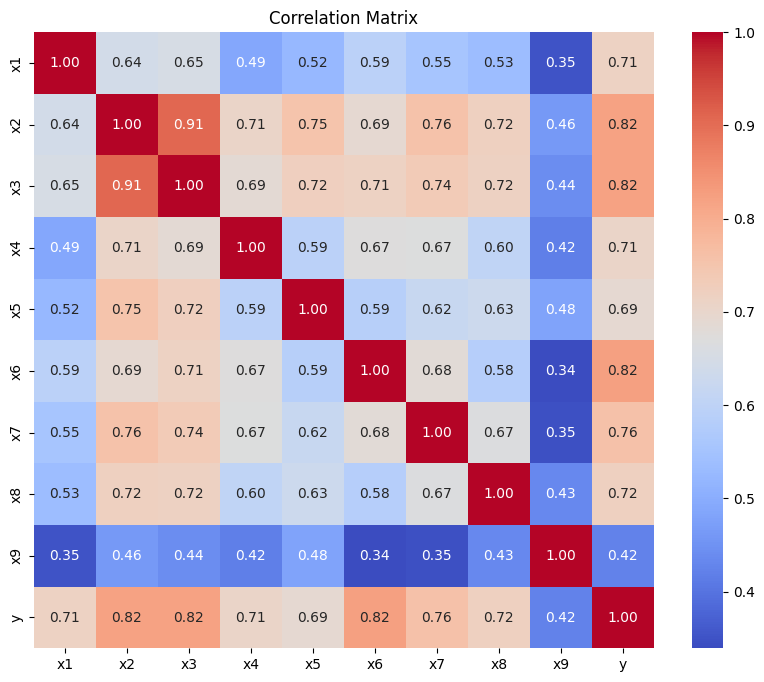
\includegraphics[width=0.7\textwidth]{corr.png} 
    \caption{Macierz korelacji Pearsona}
    \label{fig:corr}
\end{figure}

\!\!\!\!\!\!\!\!Ale zdałem sobie sprawę, że korelacja Pearsona może prowadzić do błędnych wniosków. Znalazłem test \hyperref[fig:chisq]{chi-kwadrat}, który sprawdza zależność między zmiennymi.

\begin{figure}[H]
    \centering
    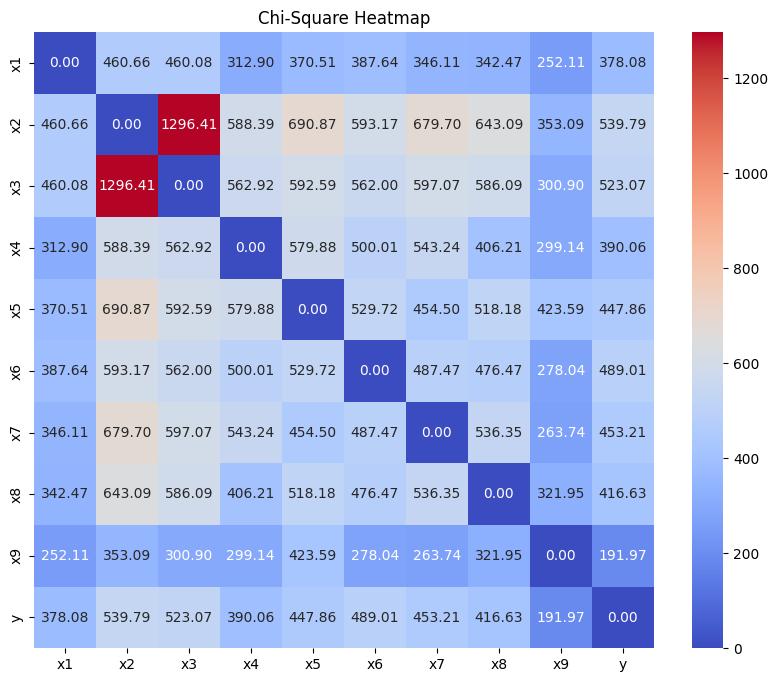
\includegraphics[width=0.75\textwidth]{chisq.png}
    \caption{Test chi-kwadrat}
    \label{fig:chisq}
\end{figure}

\!\!\!\!\!\!\!\!I dostaliśmy te same wnioski -- $x_2$ i $x_3$ są mocno zależne, a na $y$ wysoki wpływ mają $x_2, x_3$ i $x_6$. Następnie chciałem sprawdzić czy dane są liniowo separowalne i na oko \textbf{SĄ}, co odzwierciedla \hyperref[fig:pair]{kolejny wykres}. Mam świadomość, że nie jest on do końca czytelny przez rozmiar, ale po przybliżeniu widać, że w każdym kwadraciku jesteśmy w stanie narysować granicę. Jeśli popatrzymy tylko na przekątną to możemy dojść do wniosku, że  jeśli $y=2$ to $\forall j \in \{1,\dots,9\} \text{ } x_j<5$. Możemy to poprzeć już \hyperref[fig:parallel]{ostatnim wykresem}.

\begin{figure}
    \centering
    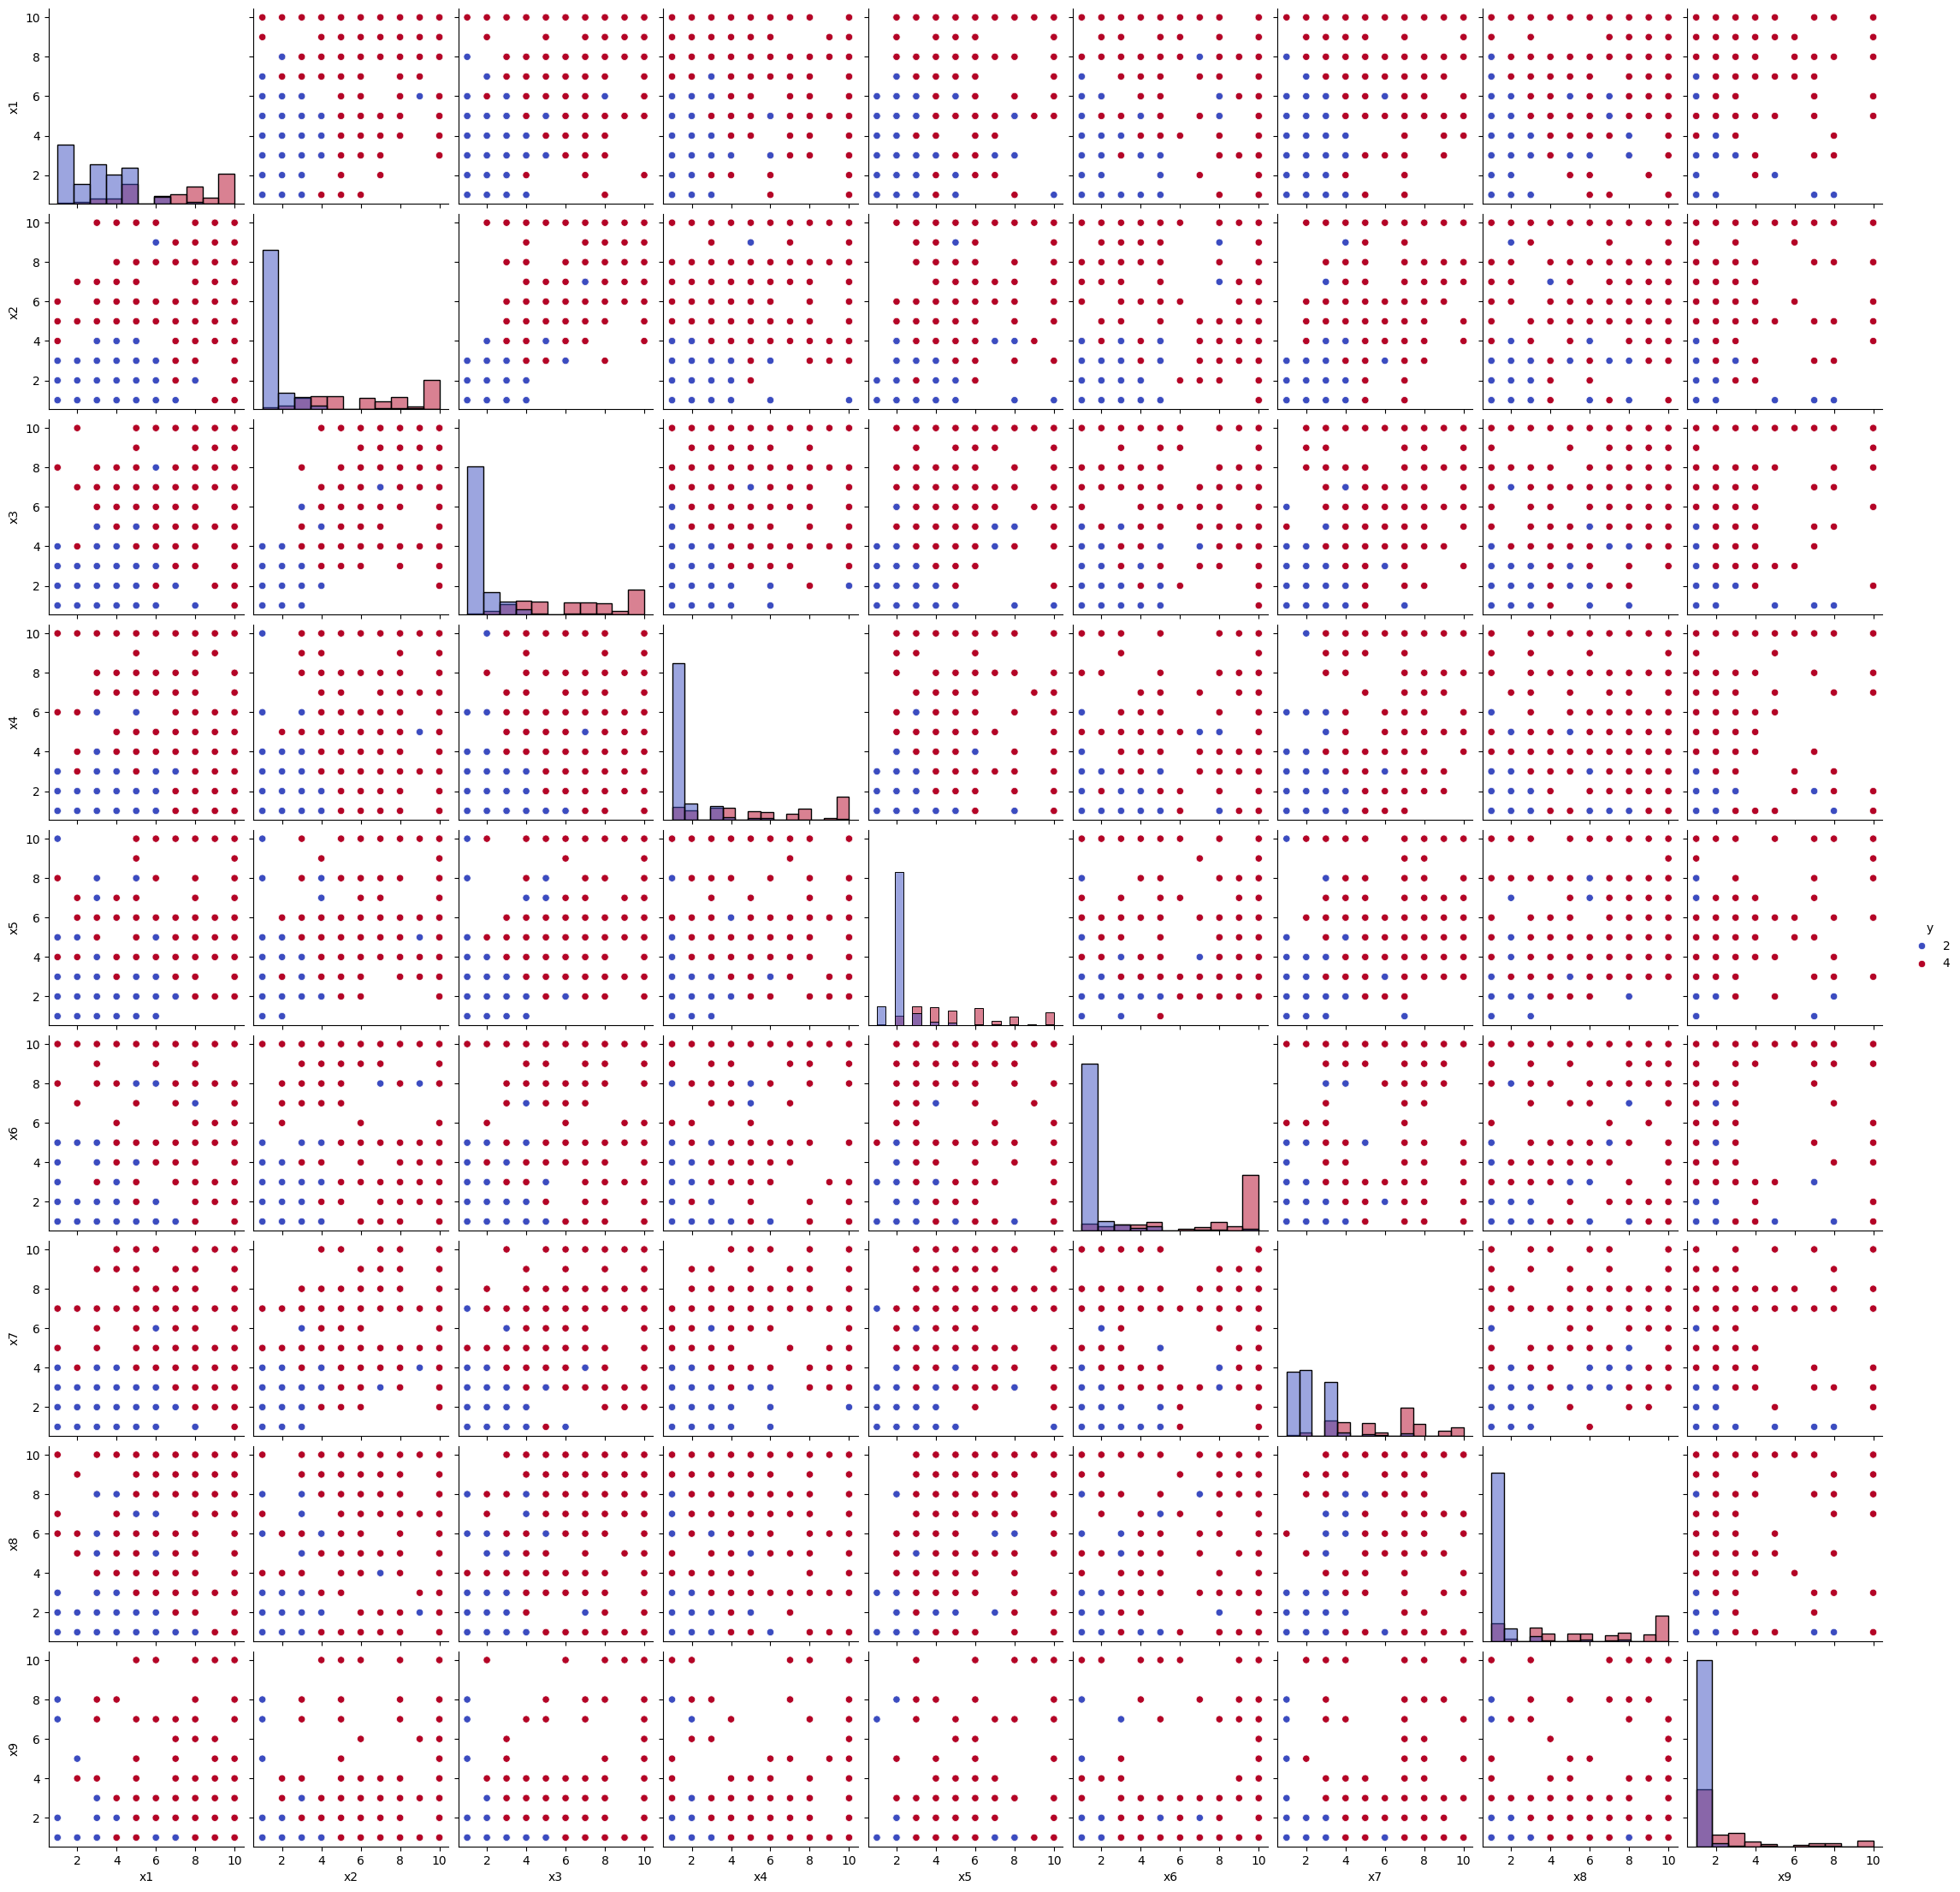
\includegraphics[width=0.9\textwidth]{pairplot.png}
    \caption{Pary zmiennych i $y$}
    \label{fig:pair}
\end{figure}

\begin{figure}[H]
    \centering
    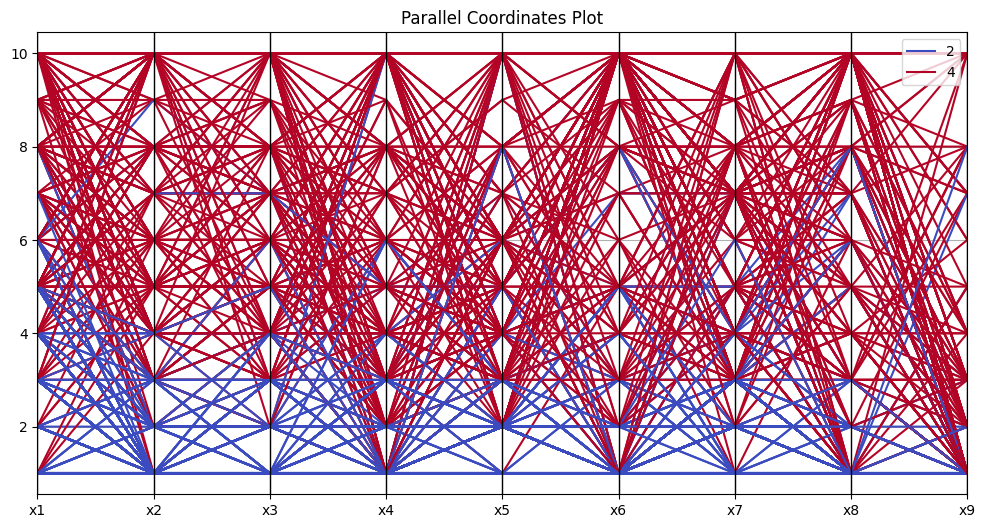
\includegraphics[width=0.7\textwidth]{parallel.png}
    \caption{Wykres równoległych współrzędnych}
    \label{fig:parallel}
\end{figure}

\section{Podział danych}
Dokonałem losowego podziału danych (67\% -- zbiór treningowy, 33\% zbiór testowy, zachowując również taki stosunek w obrębie klas $y$) 10 razy, żeby uśrednić wyniki.
Sam podział danych wygląda następująco:
\begin{algorithmic}[1]
\State $i \gets \frac{2}{3}m$
\State $XY_2 \gets \texttt{np.random.shuffle}(XY[y == 2])$
\State $XY_4 \gets \texttt{np.random.shuffle}(XY[y == 4])$
\State $\mathrm{train}_2, \mathrm{test}_2 \gets XY_2[:i], XY_2[i:]$
\State $\mathrm{train}_4, \mathrm{test}_4 \gets XY_4[:i], XY_4[i:]$
\State $\mathrm{train} \gets \mathrm{train}_2 \cup \mathrm{train}_4$
\State $\mathrm{test} \gets \mathrm{test}_2 \cup \mathrm{test}_4$
\end{algorithmic}

\section{Naiwny klasyfikator bayesowski}
Będę korzystał z wariantu z wygładzeniem Laplace'a.
\begin{align*}
    &p(y=c) = \frac{1 + \sum_{i=1}^{m}{\mathds{1}[y^{(i)} = c]}}{|C| + m} \\
    &p(x_j = d | y = c) = \frac{1 + \sum_{i=1}^{m}{\mathds{1}[y^{(i)} = c \wedge x^{(i)}_j = d]}}{|D| + \sum_{i=1}^{m}{\mathds{1}[y^{(i)} = c]}} \\
    &p(y|x) = \frac{p(x|y)p(y)}{p(x)}, \hspace{22pt} \text{co umiemy policzyć}
\end{align*}
W tym przypadku zwracamy 4, jeśli $p(y=4|x) > \frac{1}{2}$.
W implementacji nie ma żadnych trudności. Możemy usprawnić zliczanie korzystając z \texttt{np.bincount()} oraz \texttt{np.apply\_along\_axis()}. Błąd będę liczył tak jak w artykule:
\[
\texttt{error} = \frac{\sum_{i=1}^{m}{\mathds{1}[\hat{y^{(i)}} \neq y^{(i)}]}}{m}
\]
Taki naiwny klasyfikator bayesowki daje:
\begin{flalign*}
    &\texttt{Naive Bayes average error: } 0.0274 && \\
    &\texttt{Naive Bayes average training error: } 0.0214 
\end{flalign*}
Co wydaje się bardzo dobrym wynikiem. Zanim spojrzymy na dokładność, precyzję i czułość pare słów o problemach z SciKitLearnem. Biblioteka udostępnia \texttt{MultinomialNB}, który wypada gorzej niż nasz klasyfikator. 
\begin{flalign*}
    &\texttt{Sklearn Naive Bayes average error: } 0.0796 && \\
    &\texttt{Sklearn Naive Bayes average training error: } 0.1028 
\end{flalign*}
Czemu tak się dzieje? Otóż \texttt{MultinomialNB} zlicza cechy jakby one były z $\{0,1\}$. My wiemy więcej o cechach, stąd lepszy wynik. \\
Z racji tego, że badamy złośliwość raka zależy nam na wysokiej czułości.
\begin{flalign*}
    &\texttt{Naive Bayes average accuracy: } 0.9726 && \\
    &\texttt{Naive Bayes average precision: } 0.9413 && \\
    &\texttt{Naive Bayes average sensitivity: } 0.9835
\end{flalign*}
Bazowy model jest naprawdę dobry, ale co jeśli przesunęli byśmy granicę decyzyjną do $p(y=4|x) > \frac{1}{5}$.
\begin{flalign*}
    &\texttt{Naive Bayes average accuracy: } 0.9739 && \\
    &\texttt{Naive Bayes average precision: } 0.9394 && \\
    &\texttt{Naive Bayes average sensitivity: } 0.9899
\end{flalign*}
To nie jest duża poprawa, ale być może moglibyśmy wprowadzić taki hiperparametr. \\
Poniżej zamieszczam wycinek $p(y=4|x)$ dla, losowego z 10 modeli:
\begin{flalign*}
&\texttt{0.0002501727910187334}&&\\
&\texttt{0.9999955799911749}&&\\
&\texttt{0.9999999999910805}&&\\
&\texttt{0.999999999724131}&&\\
&\texttt{3.95165834865358e-09}&&\\
&\texttt{0.0002159627418231111}&&\\
&\texttt{0.9999999988067703}&&\\
&\texttt{3.95165834865358e-09}&&\\
&\texttt{0.9999999995439866}&&\\
&\texttt{1.7258835065009394e-08}
\end{flalign*}
Klasyfikator jest naprawdę pewny swoich wyborów. \\
Dodatkowo uczy się bardzo szybko, na moim komputerze średni czas uczenia:
\begin{flalign*}
&\texttt{Naive Bayes average fit time: } 0.0005753 \texttt{ seconds} &&
\end{flalign*}
Na zakończenie z Bayesem spójrzmy na wykresy uczenia z przesuniętą granicą decyzyjną.
\begin{figure}[H]
    \centering
    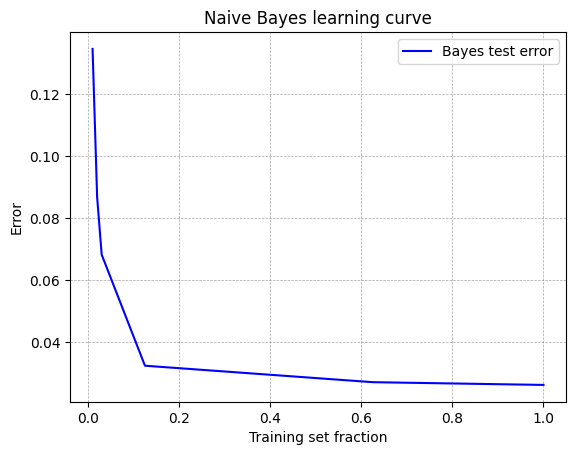
\includegraphics[width=0.75\textwidth]{naive-bayes-simple-lc.png}
    \caption{Krzywa uczenia Bayesa 1}
    \label{fig:naive-bayes-simple-lc}
\end{figure}
\begin{figure}[H]
    \centering
    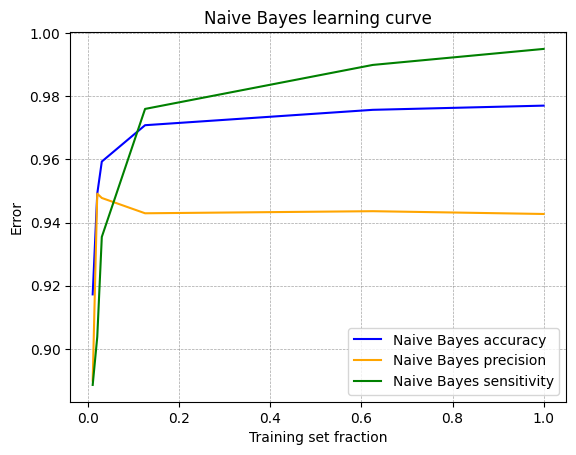
\includegraphics[width=0.75\textwidth]{naive-bayes-complex-lc.png}
    \caption{Krzywa uczenia Bayesa 2}
    \label{fig:naive-bayes-complex-lc}
\end{figure}

\section{Regresja logistyczna}
To nic innego jak obłożenie regresji liniowej \texttt{sigmoidem}.
\begin{align*}
    p(y=4|x) = \frac{1}{1 + \exp(-(\theta^T x + \theta_0))}
\end{align*}
Wynik zwracamy w taki sam sposób jak klasyfikator bayesowski. \\
Będziemy korzystać z następującej funkcji straty. 
\begin{align*}
    J(\theta) = \frac{1}{m}\sum_{i=1}^{m}{-y^{(i)}\log(\sigma(\theta^T x^{(i)} + \theta_0)) - (1 - y^{(i)})\log(1 - \sigma(\theta^T x^{(i)} + \theta_0))}
\end{align*}
Wyszedłem z założeniem, że chce użyć następującego modelu: $\theta_0$ + standaryzacja + L2 + GD, ale po drodze napotkałem okropne problemy.
\begin{enumerate}
    \item Przepisując kod na klasy (za radą Mai) pomieszałem $\hat{y}$ i $y$, co kosztowało mnie $\approx$ 1h szukania hiperparametrów gradientu na marne.
    \item Po rozwiązaniu tego problemu działała mi regresja bez $\theta_0$, bez standaryzacji i bez L2. Ona dawała kiepskie wyniki, ale takie same jak SciKitLearn.
    \begin{flalign*}
    &\texttt{Logistic regression binary cross entropy test: } 0.3863 && \\
    &\texttt{Logistic regression binary cross entropy train: } 0.4197
    \end{flalign*}
    \item Jako następny rozwiązałem problem $\theta_0$. Gradient nie mógł wejść w minimum, przez to, że pochodna po $\theta_0$ była bardzo mała w stosunku do innych pochodnych (co ma sens, ponieważ jest ona postaci $\frac{1}{m}\sum_{i=1}^{m}{\sigma(\theta^T x^{(i)} + \theta_0) - y^{(i)}}$). Najpierw dałem jej wyższą wagę -- przemnożyłem przez $m$ -- to już znacznie poprawiło zbieżność. Potem spróbowałem znormalizować gradient i to też poprawiało zbieżność. Z tych 2 pomysłów drugi wydaje się poprawniejszy formalnie, więc zostałem przy nim na chwilę.
    \begin{flalign*}
    &\texttt{Logistic regression binary cross entropy test: } 0.0657 && \\
    &\texttt{Logistic regression binary cross entropy train: } 0.1035 && \\
    &\texttt{Logistic regression error: } 0.0310 && \\
    &\texttt{Logistic regression training error: } 0.0350 && \\
    &\texttt{Logistic regression accuracy: } 0.9690 && \\
    &\texttt{Logistic regression precision: } 0.9500 && \\
    &\texttt{Logistic regression sensitivity: } 0.9620
    \end{flalign*}

    \item Teraz nastąpił przełom, ponieważ naprawiłem standaryzację -- zapomniałem zastosować skalowania w \texttt{predict()}. Otrzymujemy zawrotnie szybką zbieżność, zszedłem z 500 epok do 10.

    \item Odpuściłem już L2 patrząc na wyniki.
\end{enumerate}
Podsumowując kończymy z modelem: GD$(\alpha=0.01, \mathrm{epochs}=10)$ + standaryzacja (ta ze średnią i odchyleniem) + $\theta_0$. \\
Teraz czas na wyniki.
\begin{flalign*}
&\texttt{Logistic regression average error: } 0.0385 && \\
&\texttt{Logistic regression average training error: } 0.0298 && \\
&\texttt{Logistic regression average accuracy: } 0.9615 && \\
&\texttt{Logistic regression average precision: } 0.9551 && \\
&\texttt{Logistic regression average sensitivity: } 0.9342
\end{flalign*}
Mimo zejścia do 10 epok, regresja uczy się rząd wolniej niż naiwny klasyfikator bayesowski.
\begin{flalign*}
&\texttt{Logistic regression average fit time: } 0.0016249 \texttt{ seconds} &&
\end{flalign*}

\newpage

Na zakończenie z regresją spójrzmy na wykresy uczenia.
\begin{figure}[H]
    \centering
    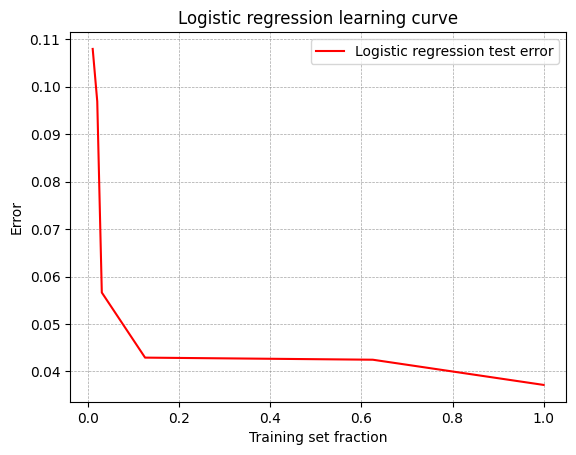
\includegraphics[width=0.75\textwidth]{reg-simple-tc.png}
    \caption{Krzywa uczenia regresji logistycznej 1}
    \label{fig:reg-simple-lc}
\end{figure}
\begin{figure}[H]
    \centering
    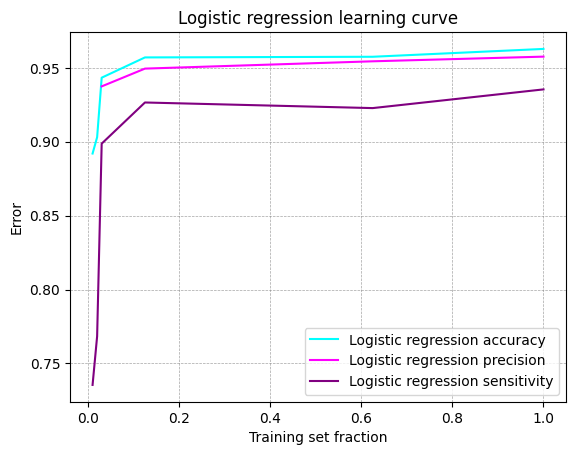
\includegraphics[width=0.75\textwidth]{reg-complex-lc.png}
    \caption{Krzywa uczenia regresji logistycznej 2}
    \label{fig:reg-complex-lc}
\end{figure}

\newpage

\section{Regresja logistyczna vs naiwny Bayes}
Naiwny klasyfikator bayesowski uczy się szybciej. Ponadto działa lepiej, co nie do końca umiem wytłumaczyć. Cechy są zależne od siebie (tak przynajmniej mówi test chi-kwadrat), ale łamią też założenie normalności, które zakłada regresja, być może jest ono silniejsze albo to ja nie umiem dobrać hiperparametrów.
\begin{flalign*}
&\texttt{Logistic regression average error: } 0.0385 && \\
&\texttt{Naive Bayes average error: } 0.0274 && \\
&\texttt{Logistic regression average accuracy: } 0.9615 && \\
&\texttt{Naive Bayes average accuracy: } 0.9739 && \\
&\texttt{Logistic regression average precision: } 0.9551 && \\
&\texttt{Naive Bayes average precision: } 0.9394 && \\
&\texttt{Logistic regression average sensitivity: } 0.9342 && \\
&\texttt{Naive Bayes average sensitivity: } 0.9899 &&
\end{flalign*}

\begin{figure}[H]
    \centering
    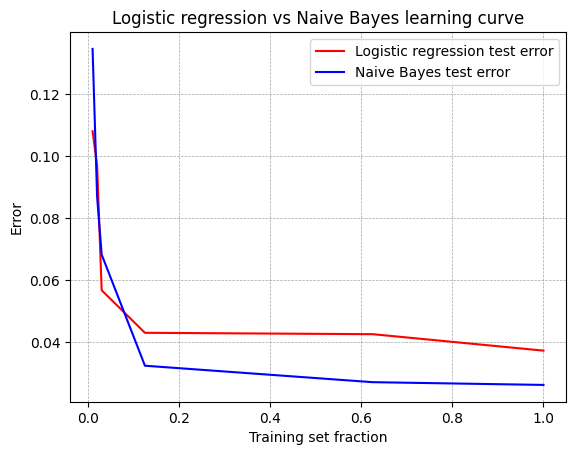
\includegraphics[width=0.75\textwidth]{reg-vs-bayes-simple.png}
    \caption{Regresja logistyczna vs naiwny Bayes 1}
    \label{fig:reg-vs-bayes-simple}
\end{figure}
\begin{figure}[H]
    \centering
    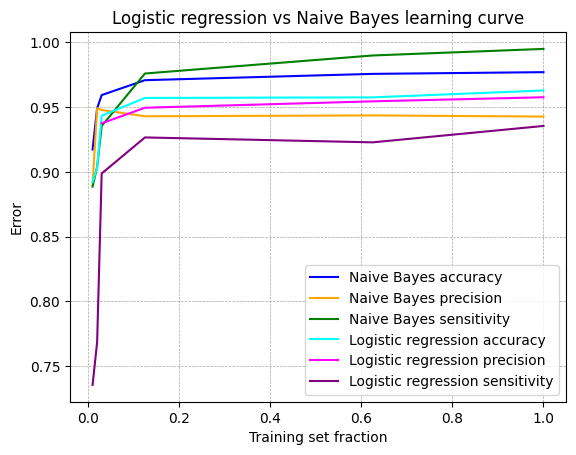
\includegraphics[width=0.75\textwidth]{reg-vs-bayes-complex.png}
    \caption{Regresja logistyczna vs naiwny Bayes 2}
    \label{fig:reg-vs-bayes-complex}
\end{figure}

\section{Jak to się ma do artykułu?}
Artykuł \textit{On Discriminative vs. Generative Classifiers: A comparison
of logistic regression and naive Bayes} Andrew Nga i Michaela Jordana wskazuje na 2 sposoby oceny modelu. Autorzy zwracają uwagę, że modele generatywne mogą być lepsze, wbrew powszechnym przekonaniom, jeśli dobierzemy odpowiednią miarę. Osiągają one swoje, co prawda wyższe, minimum znacznie szybciej. \\
U mnie tego nie widać, nie dość, że naiwny klasyfikator bayesowski okazał się lepszy, to jescze te modele zbiegają w miarę równo. Ale jest nadzieja \dots ich wykres o raku piersi również nie popiera teoretycznych wyników.
\begin{figure}[H]
    \centering
    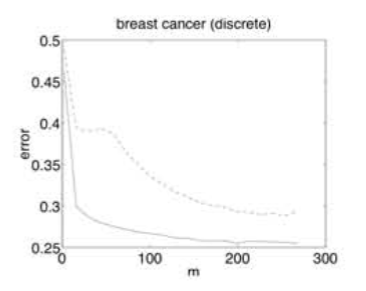
\includegraphics[width=0.4\textwidth]{breast.png}
    \caption{Wykres autorów -- przerywana linia to regresja logistyczna}
    \label{fig:breast}
\end{figure}

% Bibliography (if required)
% \bibliographystyle{plain}
% \bibliography{references}  % Add a .bib file if you have references

\end{document}